\documentclass[tikz,10pt]{standalone}
\usepackage{amsmath,amssymb,cmap,pgfplots,pgfplotstable}
\usetikzlibrary{arrows,calc,intersections}
\pgfplotsset{compat=newest}

\begin{document} 
	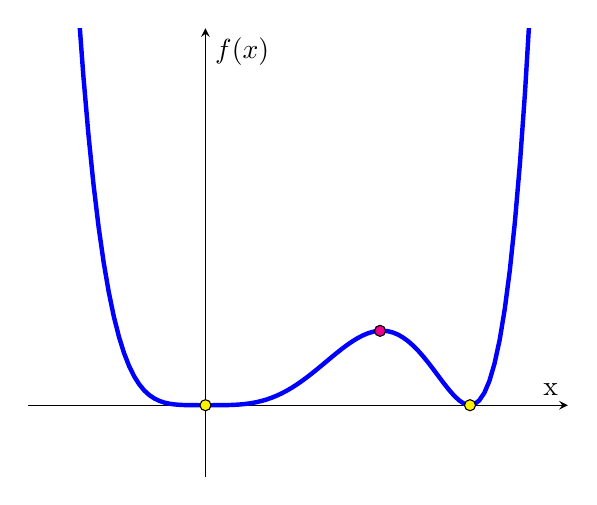
\begin{tikzpicture}
		\begin{axis}[xlabel=x, ylabel={$f(x)$}, axis lines=middle, ymax = 0.1, ymin = -0.01, xmax = 1.2,	xmin = -0.5, enlargelimits=true,xtick=\empty,	ytick=\empty]
			\addplot[blue!, line width=1.6pt,	domain={-0.5:1.4}, samples=100]{x^6-2*x^5+x^4};
			\draw[fill=yellow] (0,0) circle (2pt);
			\draw[fill=yellow] (1,0) circle (2pt);
			\draw[fill=magenta] (0.66,0.0219) circle (2pt);
		\end{axis}
	\end{tikzpicture}
\end{document}